\documentclass[12pt, a4j]{jsarticle}
\usepackage[dvipdfmx]{graphicx}
\usepackage{color, okumacro, amsmath, booktabs, colortbl, amsfonts}
\usepackage{float}

\usepackage[utf8]{inputenc}
\usepackage[expert,multi]{otf}
\input{otf-hangul.dfu}
\usepackage{palatino}


\renewcommand\thefootnote{\arabic{footnote})}

\begin{document}

\begin{center}
{\huge 政治学方法論I課題7} \\[0.2cm]
提出者:\ruby{宋}{ソン}\ruby{財\UTF{6CEB}}{ジェヒョン}(123J009J) 提出日:2014-11-17(日)
\end{center}


\section{仮説の提示}
本課題では韓国の第18代国会議員の議事堂内の座席割り当ての規定要因を分析することを目的とする。韓国の国会の座席の割り当ては基本的に自由ではあるが、同じ政党所属の議員は塊として座る傾向がある\footnote{一部の無所属議員や離党した議員は元の政党の議員たちの中に座る場合もある。}。一般的に後ろ側の座席が選好されるため、地位の高い議員たちによって占められる事が考えられる。また、同じ条件なら人気のある委員会の所属する議員たちが前列、忌避される委員会に所属する議員には後列に座らせるといった配慮があるかも知れない。したがって、本課題では以下のような仮説を検証する(モデル1)。\par

\begin{description}
	\item[仮説1] 当選回数が高い議員は後列に座る。
	\item[仮説2] 人気のある委員会に所属する議員は前列に座る。
	\item[仮説3] 忌避される委員会に所属する議員は前列に座る。
\end{description}

また、仮説2と3に関しては当選回数が高いにも関わらず、忌避委員会に所属するという事はむしろ政党内あるいは議会内での地位が低く、冷遇されると考えられるため、交互作用を考慮したもう一つもモデル(モデル2)も検証する。\par

\section{データセットの紹介}
本課題で用いるデータセットは提出者本人が作成したデータセットである。第18代国会の座席割当図は国会図書館に請求したものである。韓国の国会議事堂は10列であり、4つのブロックで分かれている。しかし、一つのブロックは7列までであるため、10点尺度で変数変換を行った\footnote{$\frac{X-1}{7-1} \times 10$}。\par
次に、議員の所属委員会は国会ホームページで入手したものである。人気委員会と忌避委員会はガ・サンジュン(2009)の議論を参考にし\footnote{ガ・サンジュン、2009「18 代国会常任委員会構成の特徴」『韓国政党学会会報』8(2)}、表~\ref{tab:委員会}のように分類を行った。\par

\begin{table}
	\centering
	\caption{第18代国会の委員会の分類} \label{tab:委員会}
	\begin{tabular}{ll}
		\toprule
		\multicolumn{1}{c}{人気委員会} & \multicolumn{1}{c}{忌避委員会} \\
		\midrule
		企画財政委員会 & 国会運営委員会 \\
		外交通商統一委員会 & 法制司法委員会 \\
		教育科学技術委員会 & 環境労働委員会 \\
		国土海洋委員会 & 女性委員会 \\
		\bottomrule
	\end{tabular}
\end{table}

その他には当選回数、年齢、女性ダミーがあり、これらは中央選挙管理委員会の選挙統計システムを参考にして作成した。ただし、当選回数が0という国会議員は存在しないため、分析の便宜のために変数変換を行った。この場合、中心化を行うと変数が小数点を持つようになり\footnote{当選回数の平均値は1.889}、解釈が不自然であると判断したため、中位数(Median)である2を引いて変換を行った。また、同様の作業を年齢にも適用した。\par

最後に地域ダミーと比例代表ダミーがある。地域ダミーは所属政党が支配的な地位を占めている地域から当選した議員のダミーである。韓国の選挙政治において地域主義\footnote{特定政党が特定地域において排他的に得票をする事。}は重要な変数であり、覇権地域から当選した候補者は首都圏などから当選した議員に比べて安易に当選でき、前列に配置されるのではないかということである。また、比例代表ダミーは比例代表で当選した議員のダミー変数であり、やはり比例代表ほど前列に配置されると思われる。\par

表~\ref{tab:記述統計}データセットの記述統計である。\par

\begin{table}[htbp]
	\centering
	\caption{変数の記述統計} \label{tab:記述統計}
	\begin{tabular}{lrrrrl}
		\toprule
		\multicolumn{1}{c}{変数} & \multicolumn{1}{c}{平均} & \multicolumn{1}{c}{最小値}& \multicolumn{1}{c}{最大値}& \multicolumn{1}{c}{標準偏差}& \multicolumn{1}{c}{}\\
		\midrule
		人気委員会 & & 0 & 1 & & 人気委員会=83; その他=160 \\
		忌避委員会 & & 0 & 1 & & 忌避委員会=52; その他=191 \\
		当選回数 & -0.111 & -1 & 4 & 1.083 & 中位数(2)を引いた変数\\
		女性 & & 0 & 1 & & 女性=32; 男性=211\\
		年齢 &  0.576 & -17 & 20 & 7.311  & 中位数(55)を引いた変数\\
		地域ダミー & & 0 & 1 & & 覇権地域=81; その他=162\\
		比例ダミー & & 0 & 1 & & PR=35; SMD=208\\
		\bottomrule
	\end{tabular}
\end{table}

\newpage

\section{分析結果}

\begin{figure}[htbp]
	\centering
	\begin{minipage}{0.4\columnwidth}
		\centering
		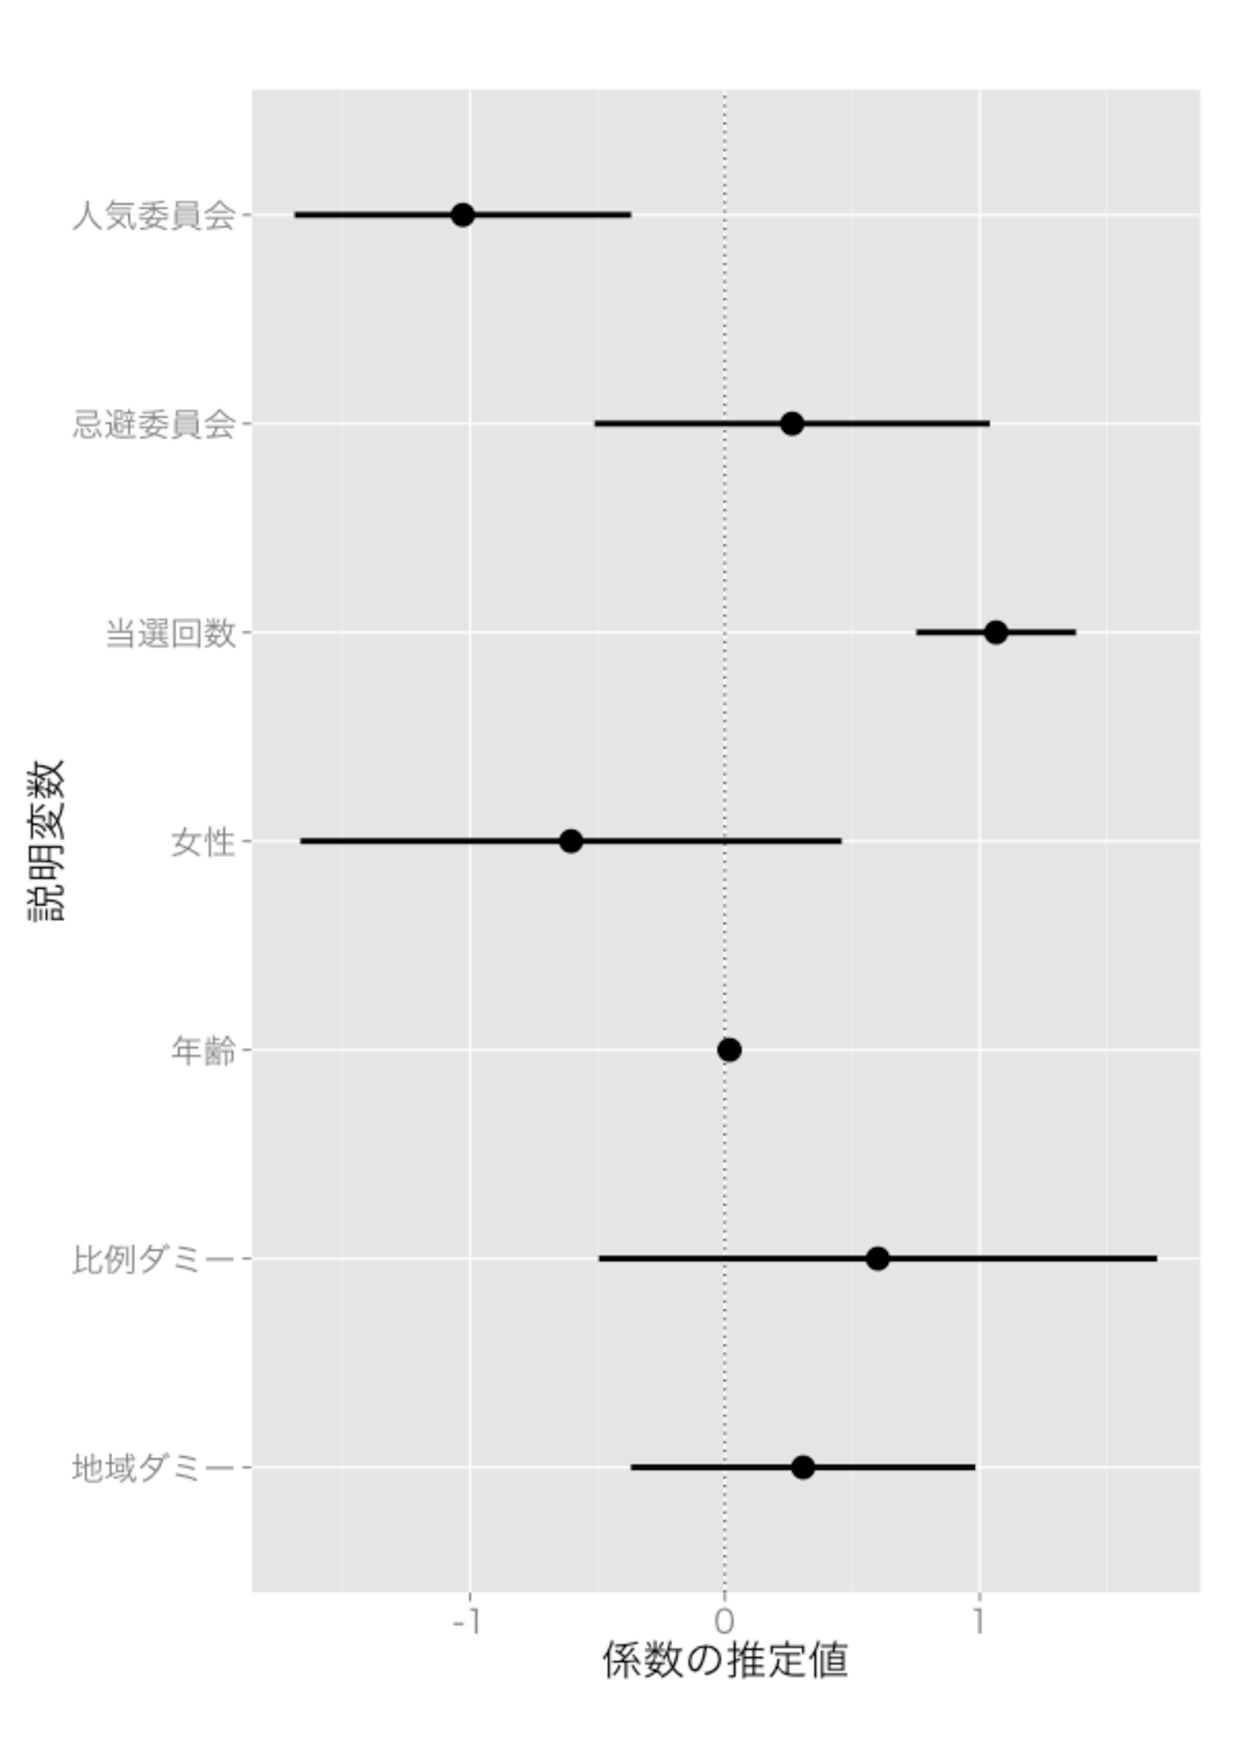
\includegraphics[width=\columnwidth]{0_figs/model1_ctplr.pdf}
		\caption{モデル2の推定値と信頼区間} \label{fig:model1_ctplr}
	\end{minipage}
	\begin{minipage}{0.4\columnwidth}
		\centering
		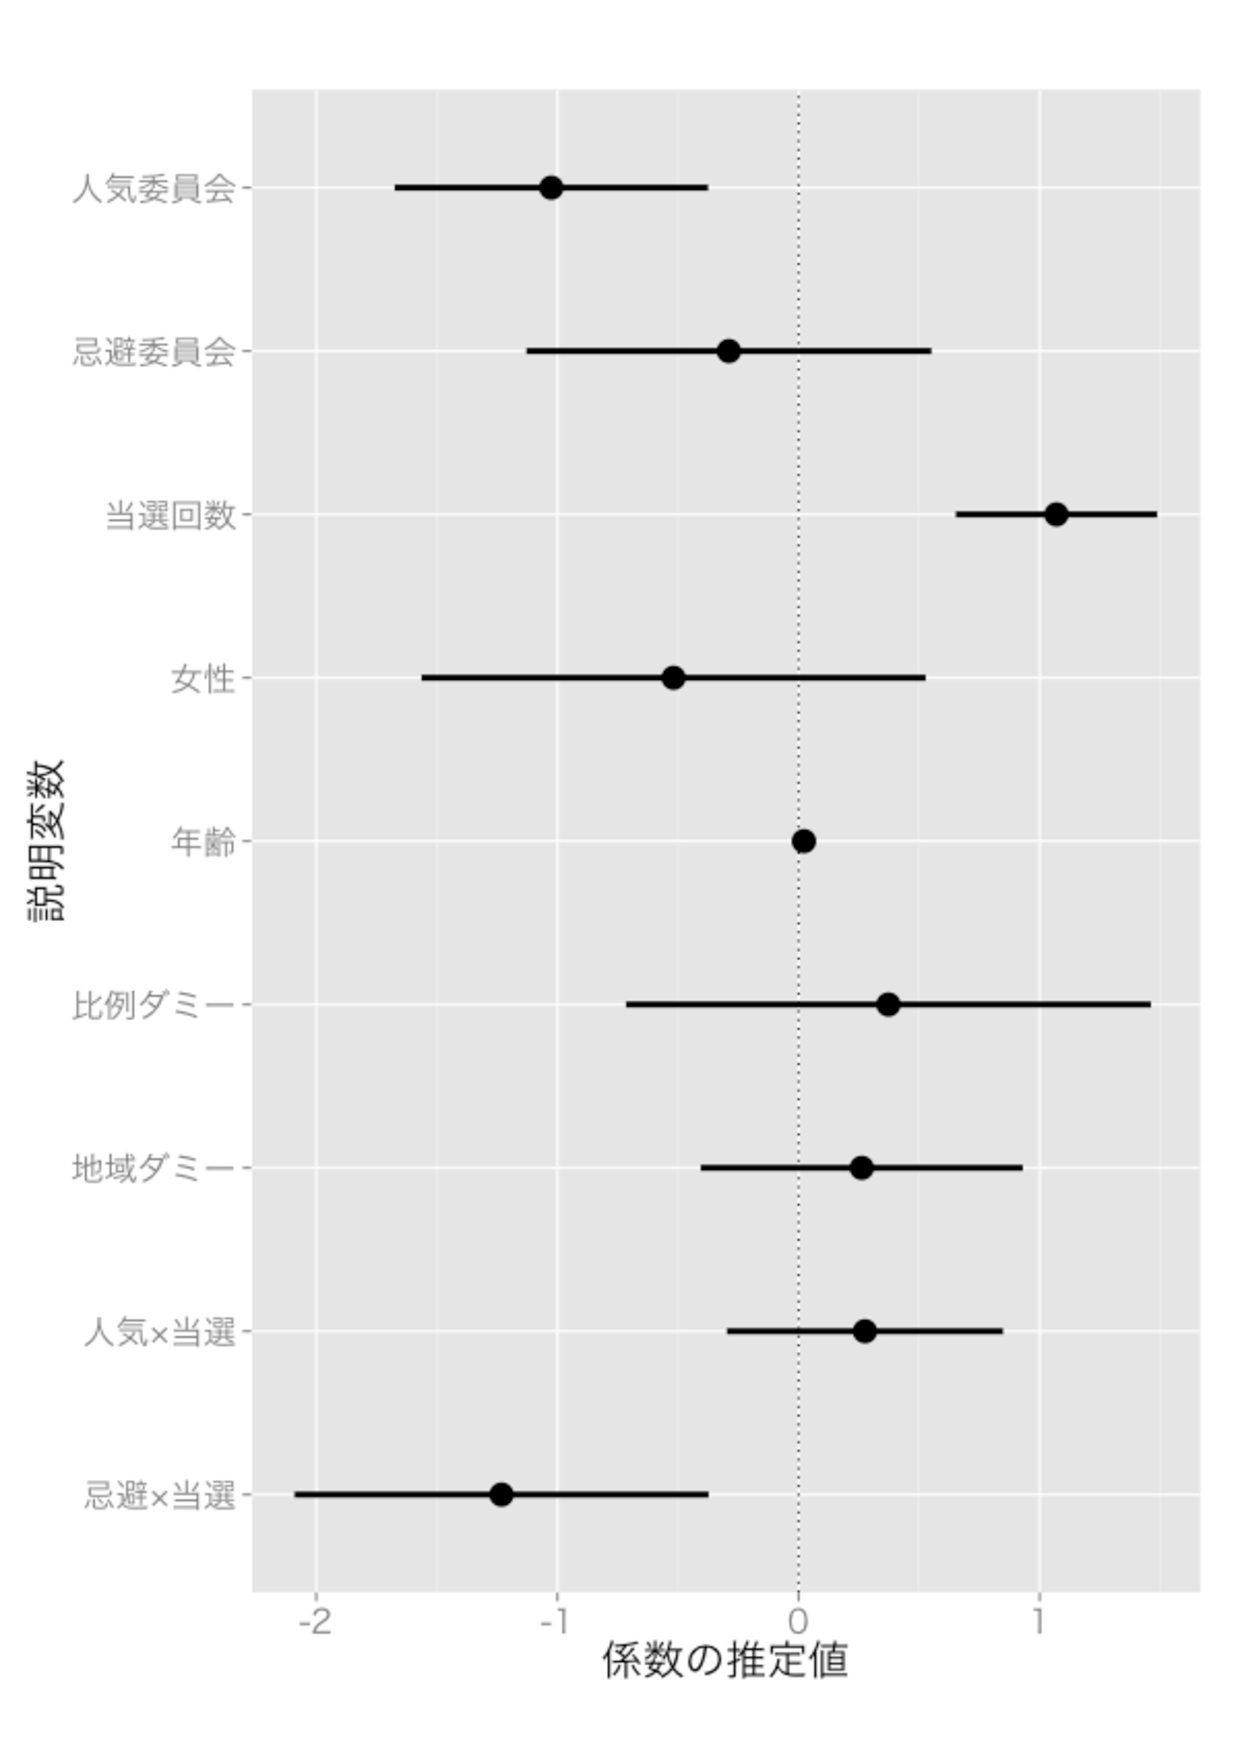
\includegraphics[width=\columnwidth]{0_figs/model2_ctplr.pdf}
		\caption{モデル2の推定値と信頼区間} \label{fig:model2_ctplr}
	
	\end{minipage}
\end{figure}

図~\ref{fig:model1_ctplr}と~\ref{fig:model2_ctplr}はモデル1とモデル2のパラメーターの推定値と信頼区間のキャタピラープロットである。全体的な傾向としては両モデルにおいて人気委員会所属ダミーと当選回数は統計的に有意な結果を示したが、忌避委員会所属に関しては統計的な有意な結果が得られなかった。忌避委員会所属に関してはモデル1では仮説とおりの方向性は示したものの、モデル2では逆の方向を示した。しかし、これらに関しては交互作用を念頭に入れた解釈が必要であろう。次に、係数の推定値の意味をより厳密に解釈するために推定値の表~\ref{tab:分析結果}で示す。\par

\begin{table}[htbp]
	\centering
	\caption{分析結果} \label{tab:分析結果}
	\begin{tabular}{lrr}
		\toprule
		& \multicolumn{1}{c}{モデル1} & \multicolumn{1}{c}{モデル2} \\
		\multicolumn{1}{c}{変数} & \multicolumn{1}{c}{係数(S.E.)} & \multicolumn{1}{c}{係数(S.E.)} \\
		\midrule
		切片& 6.799(0.263)$^{***}$& 6.810(0.259)$^{***}$ \\
		人気委員会 & -1.028(0.335)$^{**}$\textcolor{white}{$^{*}$}&  -1.025(0.330)$^{**}$\textcolor{white}{$^{*}$}\\
		忌避委員会 & 0.264(0.394)\textcolor{white}{$^{***}$}& -0.289(0.426)\textcolor{white}{$^{***}$} \\
		当選回数 & 1.065(0.159)$^{***}$ & 1.070(0.212)$^{***}$ \\
		女性 & -0.603(0.539)\textcolor{white}{$^{***}$} & -0.518(0.531)\textcolor{white}{$^{***}$}\\
		年齢 & 0.018(0.023)\textcolor{white}{$^{***}$} & 0.022(0.022)\textcolor{white}{$^{***}$}\\
		地域ダミー & 0.307(0.343)\textcolor{white}{$^{***}$} & 0.262(0.339)\textcolor{white}{$^{***}$} \\
		比例ダミー & 0.600(0.556)\textcolor{white}{$^{***}$} & 0.372(0.553)\textcolor{white}{$^{***}$} \\
		人気委員会$\times$当選回数 & & 0.275(0.291)\textcolor{white}{$^{***}$}\\
		忌避委員会$\times$当選回数 & & -1.232(0.436)$^{**}$\textcolor{white}{$^{*}$}\\
		\midrule
		$Adj. R^2$ & 0.198\textcolor{white}{$^{***}$} & 0.226\textcolor{white}{$^{***}$} \\
		AIC & 1110.699\textcolor{white}{$^{***}$} & 1104.211\textcolor{white}{$^{***}$} \\
		\midrule
		\multicolumn{3}{l}{注1: 両側検定} \\
		\multicolumn{3}{l}{注2: $^\dagger \leq 0.1{; } ^{*} \leq 0.05{; } ^{**} \leq 0.01{; } ^{***} \leq 0.001$} \\
		\bottomrule
	\end{tabular}
\end{table}

基本的にはモデル1の係数を解釈し、モデル2は交互作用を中心に解釈する。モデル1の切片は人気委員会でもなく、忌避委員会でもないその他の委員会に所属し、当選回数2回、男性、55歳、派遣地域以外の地域で当選、小選挙区で当選した議員の座席の列の期待値であり、6列から7列である。また、統計的な有意である人気委員会所属ダミー変数の係数は、他の条件が一定の場合、人気委員会に所属する議員は他の議員に比べて1列前に割り当てられると期待されるという意味である。当選回数は3回目からは当選回数が増えるにつれて大体1列後ろに割り当てられ、当選回数1回目の議員は1列前に割り当てられるということである。\par

続いてモデル2の交互作用であるが、切片の解釈は同じである。つまり、その他の委員会に所属し、当選回数2回、男性、55歳、派遣地域以外の地域で当選、小選挙区で当選した議員は6列から7列目あたりの座席に割り当てられることが期待されるという意味である。しかし、交差項として投入された人気委員会所属、忌避委員会所属、当選回数の係数は解釈が異なる。\par

\paragraph{人気・忌避委員会所属ダミー}
交互作用の構成変数の係数の意味を解釈するために、まず、表~\ref{tab:分析結果}のモデル2の回帰式を示す。\\
\begin{eqnarray}
	E[ 座席の列] & = & 6.810 - 1.025人気委員会 - 0.289忌避委員会 + 1.070当選回数 \notag \\ 
	& & - 0.518女性 + 0.022年齢 + 0.262地域ダミー + 0.372比例ダミー \notag \\
	& & + 0.275(人気委員会 \times 当選回数) - 1.232(忌避委員会 \times 当選回数) \label{eq:reg1}
\end{eqnarray}
人気委員会変数の係数である$-1.025$は$人気委員会変数 = 1$かつ、式の3列目の$0.275(人気委員会 \times 当選回数) = 0$の場合にそのままの意味を持つ。つまり$当選回数変数 = 0$、すなわち当選回数が2回の議員が人気委員会に所属する場合、1列前の座席に割り当てられるということである。忌避委員会所属の係数も同様に解釈することが出来る。\par

\paragraph{交互作用の解釈}
交互作用を検証する場合、複数の変数を総合的に見る必要がある。もし、人気委員会所属による座席割り当てが当選回数の条件付けられていると考えれば\footnote{あるいは当選回数による座席変動がどの委員会に所属しているかによって変わると考えれば}、式~\ref{eq:reg2}は以下のように表すことが出来る。\par

\begin{eqnarray}
	E[座席の列] & = & 6.810 - 1.025人気委員会 + 0.275(人気委員会 \times 当選回数) \notag \\
	& & - 0.289忌避委員会 + 1.070当選回数 - 0.518女性 + 0.022年齢 \notag \\
	& & + 0.262地域ダミー + 0.372比例ダミー - 1.232(忌避委員会 \times 当選回数) \notag \\	
	& = & 6.810 - 1.025人気委員会 + (0.275人気委員会 \times 0.275当選回数) …\notag \\
	& = & 6.810 - (1.025 - (0.275人気委員会 \times 当選回数))人気委員会 …\label{eq:reg2}
\end{eqnarray}

やや複雑になるが、人気委員会に所属すると、当選回数による期待される座席の列は$(-1.025 + 0.275)当選回数 + 1.070当選回数$だけ変わる。$人気委員会ダミー = 0$の場合は、解釈する必要がないが、もし、人気委員会に所属するならそもそも当選回数による座席に変動と当選回数によって条件付けられた人気委員会所属ダミーの係数の和、つまり$-1.025 + 1.345当選回数$だけ変わる。同様に当選回数の効果は\par

\begin{eqnarray}
	\frac{\delta 座席の列}{\delta 当選回数} & =  1.345 &\quad \text{if} 人気委員会 = 1 \notag \\
	& =  1.070 & \quad \text{if} 人気委員会 = 0 
\end{eqnarray}

である。最初の1.345は先ほど求めた値であり、1.070は当選回数変数のみの係数である。結果をより直感的に見るために、人気委員会所属による当選回数の影響をグラフとして表現すると図~\ref{fig:interaction1}のようになる。これは年齢を55歳、男性、小選挙区で当選、非覇権地域からの当選した議員を想定した上で、当選回数と人気委員会所属の有無のみを変化させた結果である。\par

\begin{figure}[htbp]
	\centering
		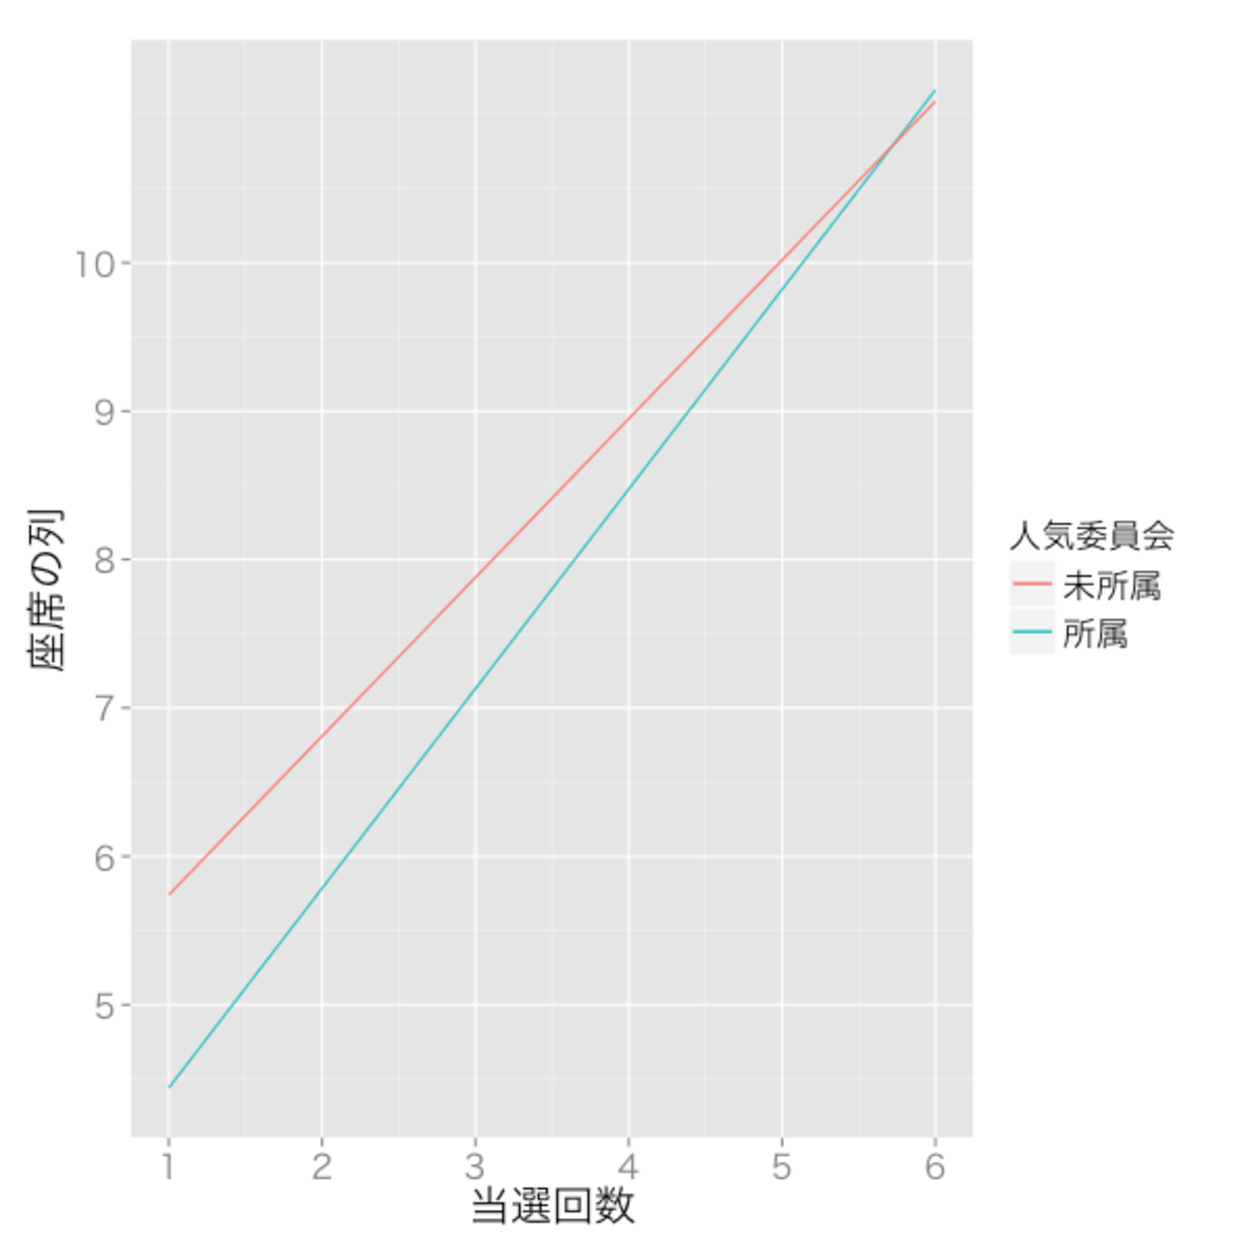
\includegraphics[width=6cm]{0_figs/interaction1.pdf}
		\caption{人気委員会所属有無による当選回数と座席の列の関係} \label{fig:interaction1}
\end{figure}

図~\ref{fig:interaction1}によると人気委員会に所属する議員はそうでない議員に比べてより前列の席に座ることが期待されるが、その差は当選回数が増えるにつれて縮まる。また、当選回数5回を超える場合、の期待値は10を超えるが、議席は最大10列であり、積極的に解釈することは難しい。次は、忌避委員会所属有無による当選回数と座席の列の関係を図示する。\par

\begin{figure}[htbp]
	\centering
		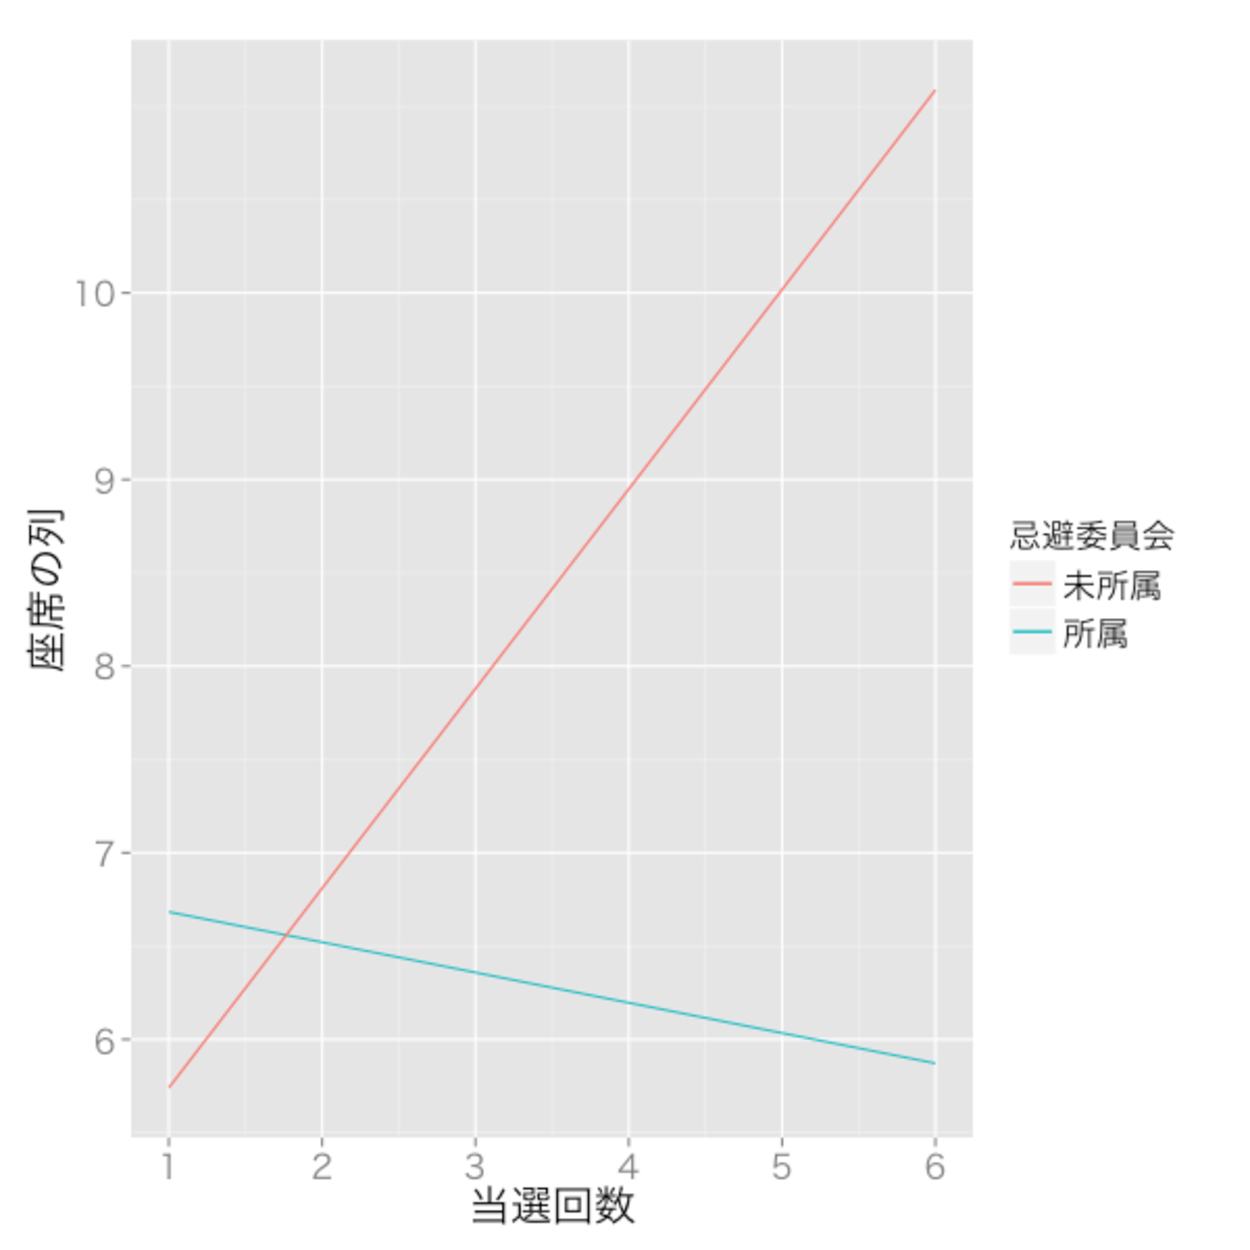
\includegraphics[width=6cm]{0_figs/interaction2.pdf}
		\caption{忌避委員会所属有無による当選回数と座席の列の関係} \label{fig:interaction2}
\end{figure}

先ほどの人気委員会所属の有無の異なり、忌避委員会所属の有無は座席の列に対して異なる方向の影響を与えることが確認できる。つまり、当選回数が1の議員は忌避委員会に所属することによって後ろの列に割り当てられると期待される。しかし、当選回数が2回以上になるとむしろ忌避委員会に所属する議員がそうでない議員よりも前列の席に割り当てられる傾向がある。しかし、この交互作用は全ての当選回数において統計的に有意であるとは断言できない。したがって、当選回数による人気・忌避委員会所属の限界効果を確認する必要があろう。例えば人気委員会所属による座席の列への影響は$-1.025 + 1.345当選回数$であり、その標準誤差は次のとおり、当選回数によって変化する。\par

\begin{gather}
	SE(\beta_{人気} + \beta_{人気 \times 当選}当選)  \notag \\
	= \sqrt{Var(\beta_{人気} + \beta_{人気 \times 当選}当選)} \notag \\
	= \sqrt{Var(\beta_{人気}) + Var(\beta_{人気 \times 当選}当選) + 2Cov(\beta_{人気}, \beta_{人気 \times 当選}当選)} \notag \\
	= \sqrt{Var(\beta_{人気}) + 当選^{2} \times Var(\beta_{人気 \times 当選}) + 2 \times 当選 \times Cov(\beta_{人気}, \beta_{人気 \times 当選})}
\end{gather}

以下の図~\ref{fig:me1}と~\ref{fig:me2}は当選回数による人気・忌避委員会所属有無の限界効果と信頼区間のグラフである。\par

\begin{figure}[htbp]
	\centering
		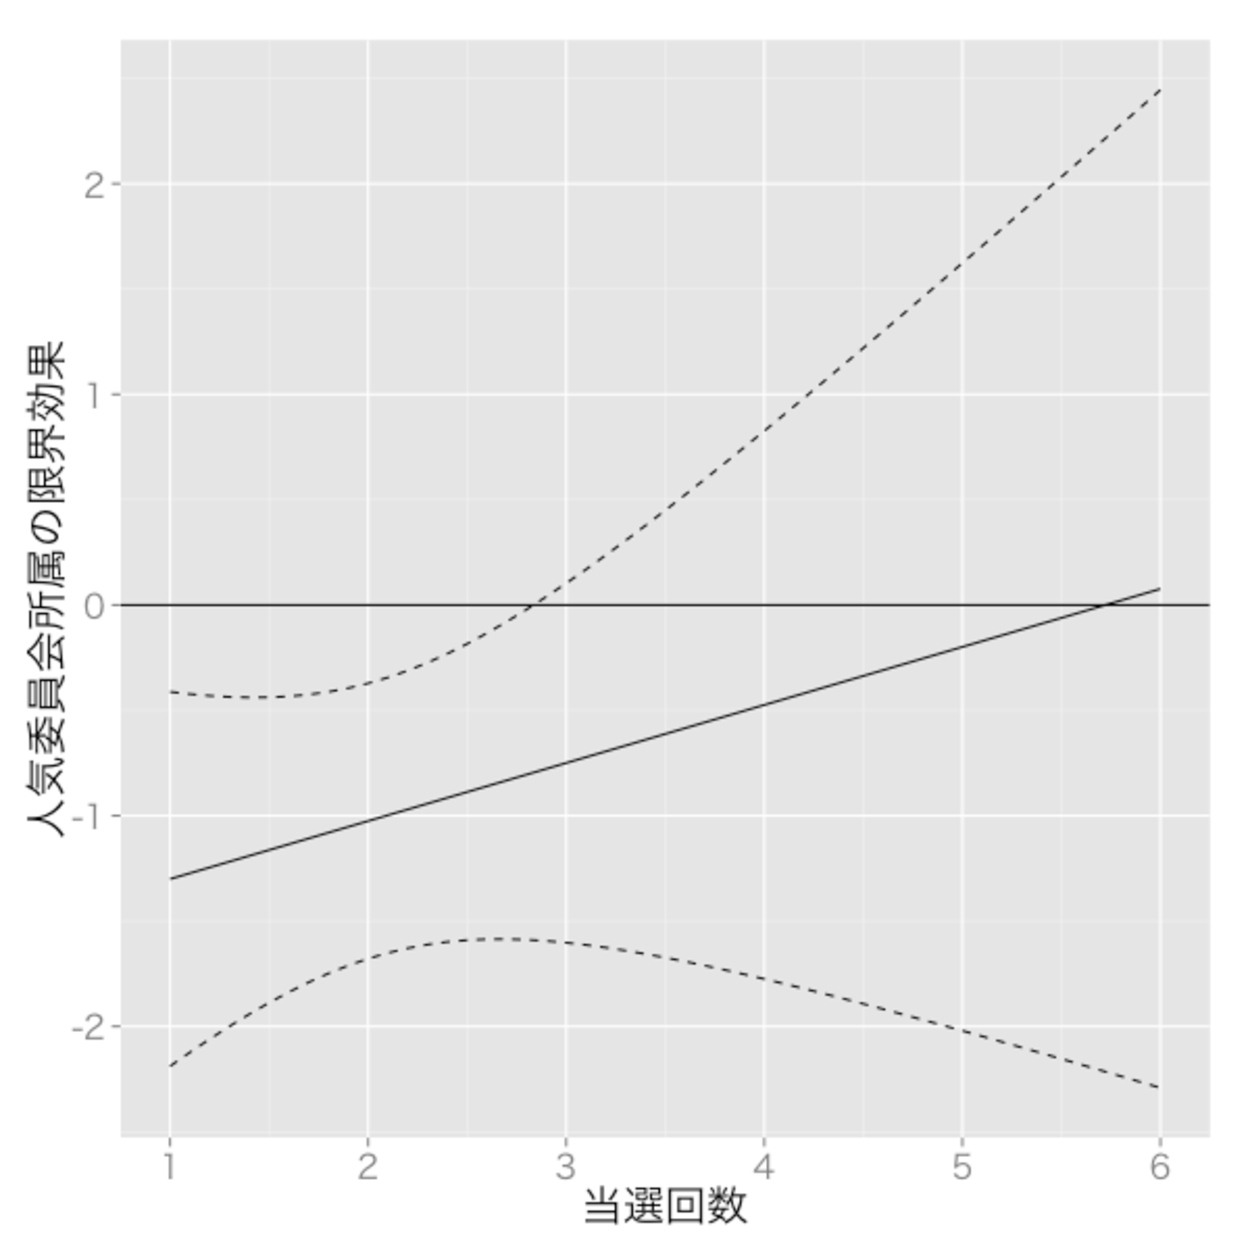
\includegraphics[width=8cm]{0_figs/meplot1.pdf}
		\caption{人気委員会所属の限界効果} \label{fig:me1}
\end{figure}

まず、人気委員会所属の限界効果を見ると全ての当選回数にわたって統計的に有意な影響を与えるのではなく、当選回数が大体3回までの議員に影響を与えることが分かる。つまり、当選回数が3回を越えると人気委員会に所属することが座席の割当に有意な影響を与えないことであり、統計的に有意である3回までを解釈すると限界効果は負の値であるため、当選回数が1、2回の議員は人気委員会に所属することによって、そうでない議員に比べて前列の座席に割り当てられることが期待できる。続いて、忌避委員会の限界効果を確認したい。\par

\begin{figure}[htbp]
	\centering
		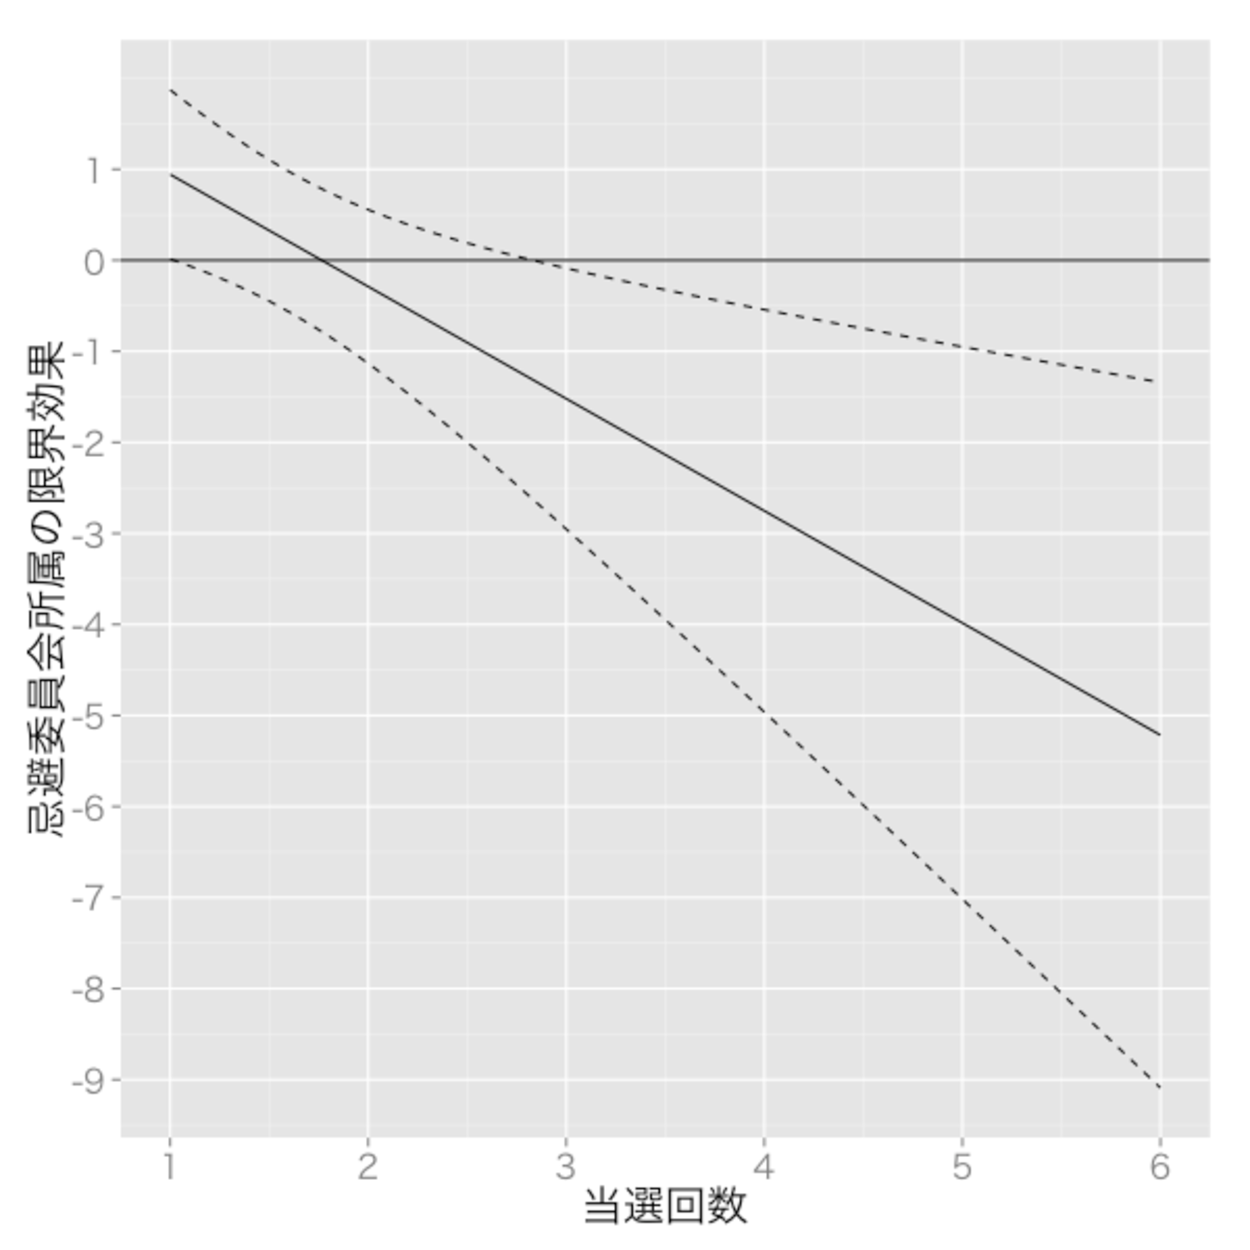
\includegraphics[width=8cm]{0_figs/meplot2.pdf}
		\caption{忌避委員会所属の限界効果} \label{fig:me2}
\end{figure}

忌避委員会所属による座席の列の変化は図~\ref{fig:interaction2}でも確認できるように、当選回数によって方向が異なる。当選回数が1回の議員は忌避委員会に所属することによって約1列後ろに割り当てられることが期待される(Lower C.I. $= 0.014$)。しかし、当選回数3回目からはむしろ前列に割りてられる傾向があり、当選回数2回は忌避委員会所属による効果は統計的には有意な影響を与えていない。\par

\end{document}
